\documentclass{article}
\usepackage{amsmath}
\usepackage{pgfplots}
\pgfplotsset{compat=newest}

\begin{document}

\begin{figure}[h]
    \centering
    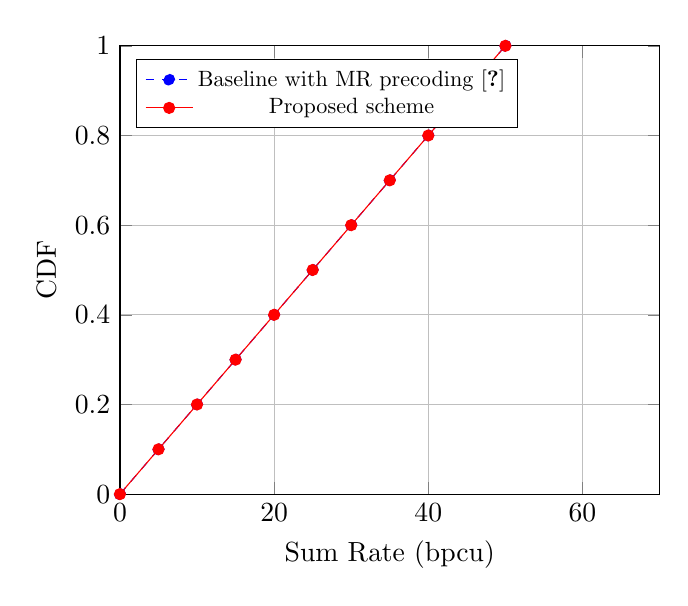
\begin{tikzpicture}
        \begin{axis}[
            xlabel={Sum Rate (bpcu)},
            ylabel={CDF},
            grid=major,
            legend pos=north west,
            xmin=0,
            xmax=70,
            ymin=0,
            ymax=1,
            xtick={0, 20, 40, 60},
            ytick={0, 0.2, 0.4, 0.6, 0.8, 1},
            legend entries={Baseline with MR precoding \cite{antonioli2023mixed}, Proposed scheme},
            legend style={nodes={scale=0.8, transform shape}},
            ]
            \addplot[blue, dashed, mark=*] coordinates {
                (0, 0) (5, 0.1) (10, 0.2) (15, 0.3) (20, 0.4) (25, 0.5) (30, 0.6) (35, 0.7) (40, 0.8) (45, 0.9) (50, 1)
            };
            \addplot[red, solid, mark=*] coordinates {
                (0, 0) (5, 0.1) (10, 0.2) (15, 0.3) (20, 0.4) (25, 0.5) (30, 0.6) (35, 0.7) (40, 0.8) (45, 0.9) (50, 1)
            };
        \end{axis}
    \end{tikzpicture}
    \caption{Performance of \gls{pcnc} scheme compared to scheme in \cite{antonioli2023mixed}. Parameters for the plot: $L=10$, $M=5$, $K=5$, and $N=1$.}
    \label{fig:performance_comparison}
\end{figure}

\end{document}